\begin{figure*}[t]
  \centering
  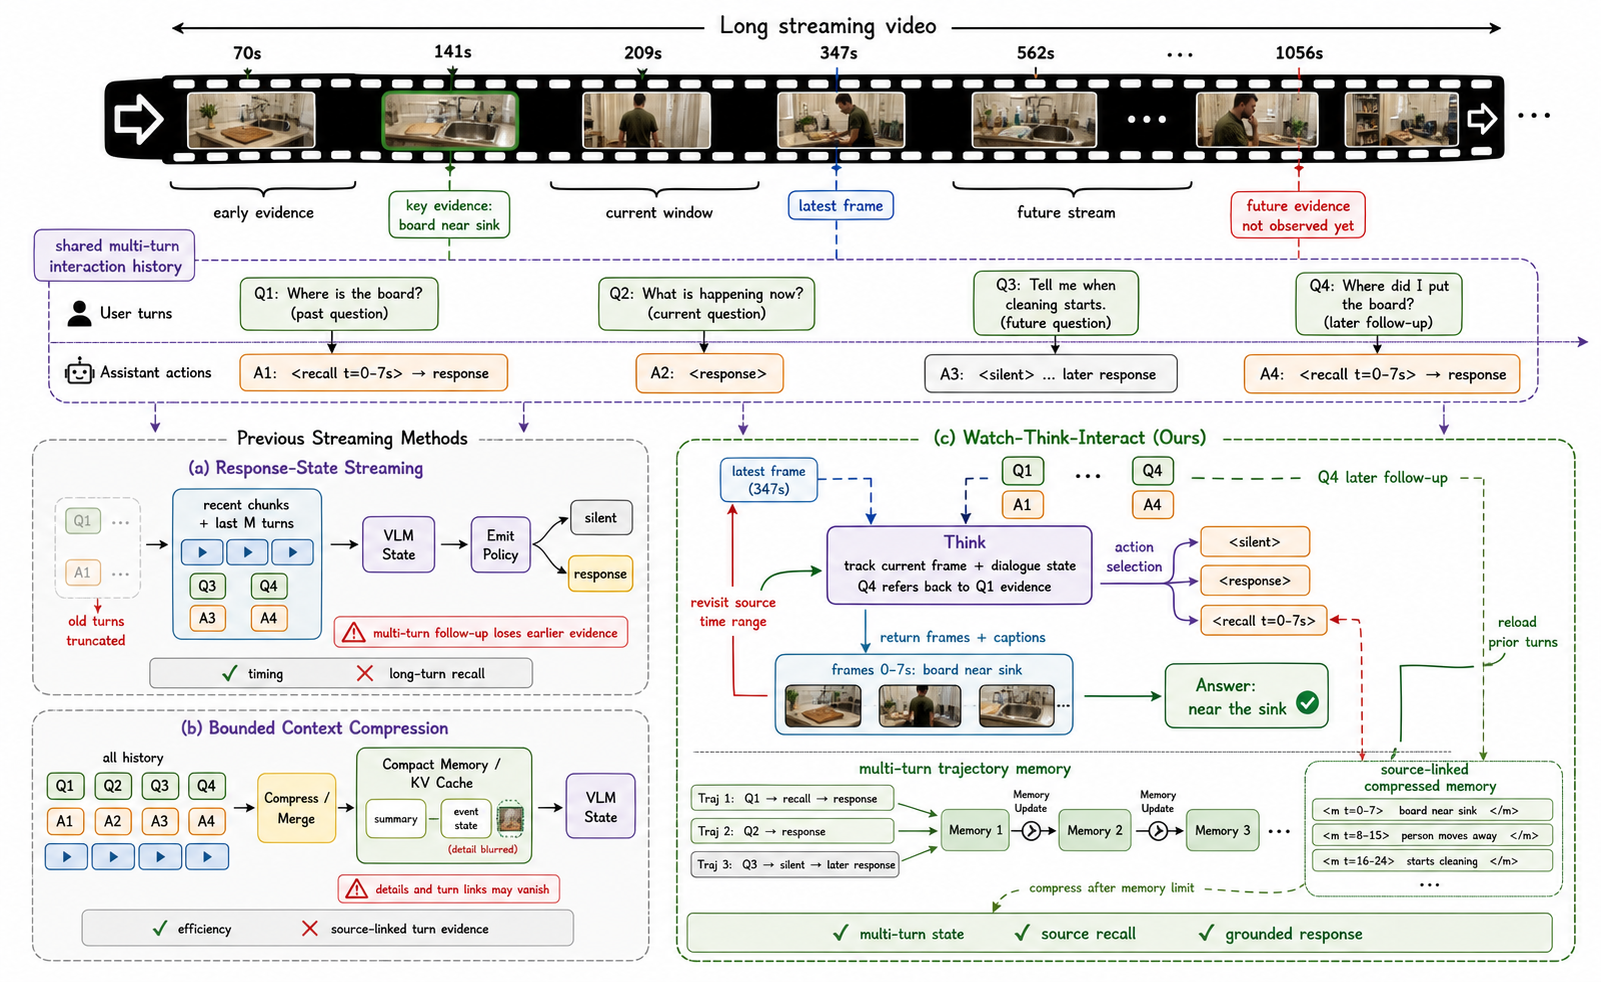
\includegraphics[width=\textwidth]{figures/figure_motivation_shared_stream.png}
  \caption{Motivation and method comparison for Watch-Think-Interact. Top: a shared streaming video with current, past, and future questions. Bottom: response-state methods lose old turns and bounded compression may blur earlier evidence, while WTI maintains multi-turn state, compact time-indexed memory, and time-bounded recall.}
  \label{fig:chronostream-motivation}
\end{figure*}

\section{Introduction}

Recent Video Large Language Models (Video-LLMs) have made progress in offline video question answering, long-video understanding, and temporal reasoning~\citep{mvbench2024,longvideobench2024,videomme2025}.
Yet most methods assume access to a full video or pre-collected clip before inference.
Streaming scenarios break this assumption.
Frames arrive continuously, queries may arise anytime, and future frames are unavailable.
Thus, a streaming model must maintain its history under finite context and low-latency constraints.
This history must retain early evidence for later turns, even after that evidence leaves the active visual context.

Recent streaming Video-LLMs adapt offline video models for continuous interaction.
They model response states or online decisions over observed prefixes~\citep{videollm_online2024,dispider2025,vispeak2025}, and introduce timestamped interaction, proactive responses, or streaming instruction data~\citep{livecc2025,streamo2026,streambridge2025,livestar2025}.
They improve streaming interaction but mainly judge whether the active window suffices for the next output.
Thus, their state favors timely responses and struggles with long-range dependencies once evidence for later verification leaves the active window.

Another line of work targets context cost, making long streams tractable through KV/cache management and recurrent state control~\citep{streamingvlm2026,flashvstream2025}.
Visual-token compression, hierarchical compression, and event-level memory further reduce dense video context~\citep{longvu2025,videochatflash2026,streamforest2025}.
Yet forward-only compression has intrinsic limits.
The model decides what enters compressed memory from the current state, but an early segment may become important only after later questions or observations appear.
Meanwhile, repeated compression and overwriting gradually remove fine-grained details that later turns may need to inspect.

Motivated by this gap, we introduce Watch-Think-Interact, an end-to-end framework for long-horizon multi-turn streaming video reasoning.
As the stream unfolds, the model updates a chunk-level thinking state and chooses to stay silent, answer, or recall time-bounded historical evidence outside the active window.
When context reaches its limit, it performs compact state transfer by rewriting observed history into time-indexed memory lines and continuing from the compact state.
Together, these actions form a single online trajectory that lets the model update state, make interaction decisions, and process potentially unbounded streams under a fixed context budget.

To train Watch-Think-Interact, we construct ChronoInteract-82K, a dataset of chunk-level streaming interaction trajectories built under strict streaming causality.
These trajectories supervise interaction decisions and context-bounded state updates.
SFT initializes the interaction format, while Stream-GDPO optimizes online rollouts for answer correctness, response timing, evidence use, and long-range history maintenance.
Experiments show that WTI reaches 83.3\% on StreamingBench~\citep{streamingbench2024} and 73.6\% on OVO-Bench~\citep{ovobench2025}, achieving state-of-the-art streaming performance while preserving competitive long-video understanding~\citep{longvideobench2024}.

In summary, our contributions are as follows:
\begin{itemize}[leftmargin=*, itemsep=1pt, topsep=1pt, parsep=1pt, partopsep=1pt]
  \item We introduce Watch-Think-Interact, a closed-loop framework unifying watching, thinking, response timing, historical recall, and compact state transfer for long-horizon multi-turn streaming video reasoning under bounded context.
  \item We construct ChronoInteract-82K, aligning video chunks, asynchronous queries, answerable moments, and evidence dependencies on a shared timeline for streaming interaction training under causal timing.
  \item We propose Stream-GDPO, a trajectory-level GDPO objective optimizing answer correctness, response timing, evidence use, and long-range history maintenance in the same chunk-level online environment.
  \item WTI achieves state-of-the-art streaming performance, reaching 83.3\% on StreamingBench and 73.6\% on OVO-Bench, with ablations verifying the roles of recall, compact state transfer, and training design.
\end{itemize}
